\input{../common}
\everymath{\displaystyle}
\begin{document}
  %<*content>
  \lesson{algebra}{5}{Fonction exponentielle (TS2)}

 \subsection*{Introduction}
  $ \text{La fonction } \;\;\begin{array}{lrcl}
\ln : & \intoo{0}{\pinf} & \longrightarrow & \Rr \\ 
      & x                & \longmapsto     & \ln x
\end{array} \;\text{est continue et strictement croissante.}$
    
    
 Elle admet une    \textbf{ bijection  réciproque } de $\; \Rr  \;$ vers $\;\intoo{0}{\pinf} $.

\subsection{Définition et propriétés}

\begin{definition}
On appelle fonction  exponentielle,  notée     exp  ou e, la bijection réciproque de la fonction $ \ln $.
\end{definition}

\begin{notation}
 $$ \begin{array}{lrcl}
\text{exp} : & \Rr & \longrightarrow & \intoo{0}{\pinf} \\
             & x   & \longmapsto     & \text{exp}(x) = \eexp{x}
\end{array} $$
\end{notation}
\begin{corollary}
\begin{itemize}
\item $ \forall x \in \Rr,\; \; \eexp{x}> 0 $ 

\item $  \eexp{0}= 1   \; $ et $ \;    \eexp{1}= \mathrm{e} $

 \item $\forall x> 0,\; \; \eexp{\ln{x} }=x  $ 
 
 \item $\forall y\in \Rr ,\; \; \ln {\eexp{y}}=y  $ 
  
  \item exp   est continue et dérivable sur  $\Rr$.
  \item exp   est bijective et  strictement croissante  sur $\Rr$. D'où :
  
  \item $ \eexp{a}=\eexp{b}\Longleftrightarrow a=b $
  
\item $ \eexp{a}> \eexp{b}\Longleftrightarrow a>b $
 
\end{itemize}

\end{corollary}


\begin{property}[fondamentale]

$$ \forall a \in \Rr \; \text{et} \;  \forall b \in\Rr: \quad \eexp{a+b}=\eexp{a}\times \eexp{b}  $$


\end{property}

\textbf{Démonstration}\\
$ \ln \paren{\eexp{a+b}}  =a+b $  \\
$  \ln \paren{\eexp{a} \times \eexp{b}}=\ln (\eexp{a})+ \ln {\eexp{b}} =a+b$ \\  D'où $ \;\;\eexp{a+b}=\eexp{a}\times \eexp{b}  $  

\begin{corollary}
 \begin{itemize}
 \item $ \eexp{-a}=\dfrac{1}{\eexp{a}} $
  \item $ \eexp{a-b}=\dfrac{\eexp{a}}{\eexp{b}} $
  
  \item $ \paren{\eexp{a}}^{r} = \eexp{ra} \quad \forall r \in \Qq $
 \end{itemize}
\end{corollary}


\subsection{Étude et représentation graphique}
Les  courbes de la fonction   exp   et de la fonction $ \ln  $ sont symétriques  par  rapport à la première bissectrice du repère.
  \begin{center}
\begin{tikzpicture}[>=stealth', scale=0.5]
\clip (-4,-3) rectangle (7,7);
\draw[->,thick] (0,0) -- (1,0);
\draw[->,thick] (0,0) -- (0,1);
\draw[,thick] (-4,0) -- (7,0);
\draw[thick] (0,-3) -- (0,7);
\foreach\x in {1,2,}
{
\draw[thick] (\x,0.1) -- (\x,-0.1) node[below] {\x};
}
\foreach\y in {1}
{
\draw[thick] (0.1,\y) -- (-0.1,\y) node[left] {\y};
}

\draw[thick,black] plot[domain=0.1 :7,samples=100] (\x,{ln (\x)}) node[above left] {$\mathscr{C_{\ln}}$};
\draw[thick,black] plot[domain=-3 :1.78,samples=100] (\x,{exp (\x)}) node[above left] {$\mathscr{C_{\exp}}$};
\draw[thick,dashed] plot[domain=-3 :7,samples=100] (\x, \x);
\draw[dashed,thick](2.7,0)--(2.7,1);
\draw[dashed,thick](2.7,1)--(0,1);
\node at(2.7,-0.4) {$\mathrm{e}$};
\node at(-0.4, 2.7) {$\mathrm{e}$};
\draw[dashed,thick](0,2.7)--(1,2.7);
\draw[dashed,thick](1,2.7)--(1,0);

\end{tikzpicture}
\end{center}


\subsection*{Limites} 
Aux bornes de l'ensemble de définition de la fonction exp, on obtient les limites suivantes:
\begin{property}
\begin{itemize}
\item  $\displaystyle \lim_{x \to \pinf}\eexp{x} =\pinf $ 
 \item $ \displaystyle\lim_{x \to \minf}\eexp{ x}=0 $
\end{itemize}
\end{property}

\textbf{Démonstration}
\begin{itemize}
\item  Soit $ \varphi $  la fonction définie par : $\; x\longmapsto \eexp{x}-x-1 $. \\
$ \varphi $  est dérivable sur $ \intfo{0}{\pinf} \;$    et  $ \;\forall x> 0 \quad  \varphi^{\prime}(x)= \eexp{x}-1\geq 0$.  $ \;\varphi $  est donc croissante sur  $ \intfo{0}{\pinf} \;$    or  $ \;\varphi(0)=0. $  \\ Donc $ \forall x \geq 0,\; \varphi(x)\geq 0 \;$  càd  $ \eexp{x}\geq x+1 $.  Or $ \displaystyle\lim_{x \to \pinf}x+1=\pinf $  
par comparaison  $ \displaystyle\lim_{x \to \pinf}\eexp{x} =\pinf $ \\
\item Pour calculer $ \displaystyle\lim_{x \to \minf}\eexp{ x} $\;  posons\; $ y=-x $   \\
On a alors \;$\displaystyle\lim_{x \to \minf}\eexp{ x} = \displaystyle\lim_{y \to \pinf}\eexp{-y}=\lim_{y \to \pinf}\dfrac{1}{\eexp{y}}=0 $

\end{itemize}
\subsection*{ Tableau de variations}
\begin{center}
\begin{tikzpicture}
\tkzTabInit[lgt=1.5,espcl=1]
{$x$ /1, $(e^x)'$ /1, $e^x$ /1.5}
{$-\infty$, $+\infty$}

\tkzTabLine{, +, }

\tkzTabVar{-/$0$, +/$+\infty$ , }
\end{tikzpicture}


\end{center}

\subsection*{Dérivée} 
On sait que  $\; \forall x \in \Rr ,\;  \ln{\eexp{x}}=x $. \\
Dérivons les 2 membres de cette égalité.  \\
$ \ln^{\prime}\paren{ \eexp{x}}\times \paren{\eexp{x}}^{\prime}=1$ \\
$ \dfrac{\paren{\eexp{x}}^{\prime}}{\eexp{x}}=1   \Longleftrightarrow  \paren{\eexp{x}}^{\prime}=\eexp{x}$ 

\begin{property}
 La fonction exponentielle est dérivable sur $ \Rr $ et est égale à sa propre dérivée:
 $ \paren{ \eexp{x}}^{\prime}=\eexp{x}\;\;  \quad \forall x \in \Rr $
\end{property}
\begin{corollary}
Si $u$ est une fonction  dérivable sur un intervalle I alors la fonction $\; f: x \mapsto \eexp{u(x)} \;$  est dérivable sur I  et  $ f'(x)=\paren{\text{exp}^{\prime}(u(x))}\times u'(x) = \eexp{u(x)}\times u'(x)=\eexp{u(x)}\times u'(x)$ 

 \fbox{$ \paren{\eexp{u}}^{\prime}= u^{\prime} \eexp{u}$}
\end{corollary}

 La fonction  $\;  u^{\prime}\eexp{u} \;$  a pour primitive   sur I, toute fonction du type  $\;  \eexp{u}+C \; $ $ (C\in\Rr) $.
 


\subsection{ Quelques limites classiques}

\begin{property}
\begin{itemize}
\item  $\displaystyle \lim_{x \to \pinf}\dfrac{\eexp{x}}{x}=\pinf $
\item  $\displaystyle \lim_{x \to \minf} x\eexp{x}=0 $   
\item  $\displaystyle \lim_{x \to 0} \dfrac{\eexp{x}-1}{x}=1 $
\end{itemize}
\end{property}


\textbf{Démonstration}
\begin{itemize}
\item   Montrons que $ \displaystyle\lim_{x \to \pinf}\dfrac{\eexp{x}}{x}=\pinf $ \\  
 Pour $ x > 0 $,\; $ \ln  \paren{\dfrac{\eexp{x}}{x}}  =\ln \eexp{x}-\ln x  =x-\ln x  =x\paren{1-\dfrac{\ln x}{x}}\; $   d'où par produit  $\displaystyle \lim_{x \to \pinf}x\paren{1-\dfrac{\ln x}{x}}=\pinf $
 
 \item   Montrons que\; $ \displaystyle\lim_{x \to \minf}x\eexp{x}=0 $ \\\ 
 En posant $ X=-x $ ,\;on obtient $\displaystyle \lim_{x \to \minf}x\eexp{x}=\lim_{X \to \pinf}-X\eexp{-X} = \displaystyle\lim_{X \to \pinf}\dfrac{-X}{\eexp{X}}=0$ 
 \item  Montrons que\; $ \displaystyle\lim_{x \to 0} \dfrac{\eexp{x}-1}{x}=1 $\\
  Soit $ \varphi (x)=\eexp{x}$.\\
  $\displaystyle \lim_{x \to 0}  \dfrac{\eexp{x}-1}{x} =\displaystyle\lim_{x \to 0}  \dfrac{\varphi(x)-\varphi(0)}{x-0} = \varphi'(0)=\eexp{0}=1$
  \end{itemize}




  %</content>
\end{document}
